\tikzset{every picture/.style={line width=0.75pt}} %set default line width to 0.75pt        

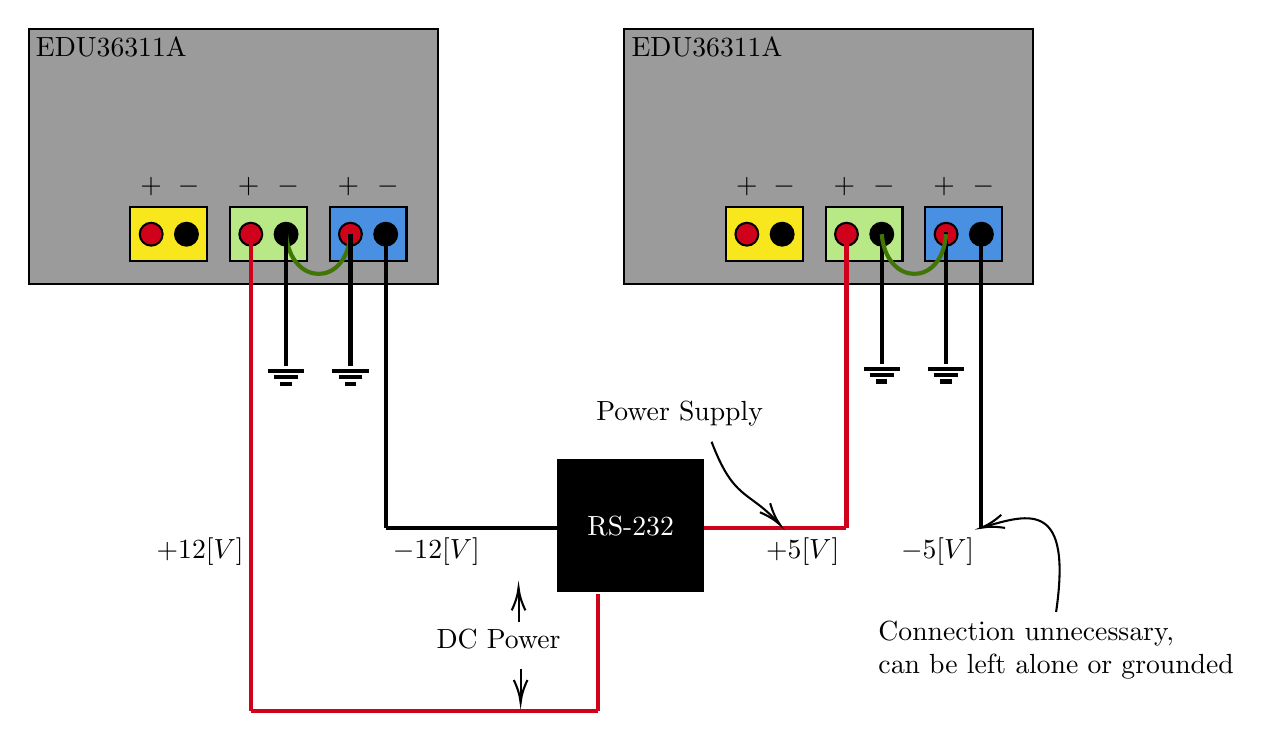
\begin{tikzpicture}[x=0.75pt,y=0.75pt,yscale=-1,xscale=1]
%uncomment if require: \path (0,437); %set diagram left start at 0, and has height of 437

%Shape: Rectangle [id:dp40376072703618315] 
\draw  [fill={rgb, 255:red, 155; green, 155; blue, 155 }  ,fill opacity=1 ] (43,81) -- (240,81) -- (240,204) -- (43,204) -- cycle ;
%Shape: Rectangle [id:dp9680918137452028] 
\draw  [fill={rgb, 255:red, 74; green, 144; blue, 226 }  ,fill opacity=1 ] (188,167) -- (225,167) -- (225,193) -- (188,193) -- cycle ;
%Shape: Rectangle [id:dp46673703877752515] 
\draw  [fill={rgb, 255:red, 184; green, 233; blue, 134 }  ,fill opacity=1 ] (140,167) -- (177,167) -- (177,193) -- (140,193) -- cycle ;
%Shape: Rectangle [id:dp1742550836975566] 
\draw  [fill={rgb, 255:red, 248; green, 231; blue, 28 }  ,fill opacity=1 ] (92,167) -- (129,167) -- (129,193) -- (92,193) -- cycle ;
%Shape: Circle [id:dp5502231665626698] 
\draw  [fill={rgb, 255:red, 208; green, 2; blue, 27 }  ,fill opacity=1 ] (96.5,180) .. controls (96.5,176.96) and (98.96,174.5) .. (102,174.5) .. controls (105.04,174.5) and (107.5,176.96) .. (107.5,180) .. controls (107.5,183.04) and (105.04,185.5) .. (102,185.5) .. controls (98.96,185.5) and (96.5,183.04) .. (96.5,180) -- cycle ;
%Shape: Circle [id:dp39831821955516866] 
\draw  [fill={rgb, 255:red, 0; green, 0; blue, 0 }  ,fill opacity=1 ] (113.5,180) .. controls (113.5,176.96) and (115.96,174.5) .. (119,174.5) .. controls (122.04,174.5) and (124.5,176.96) .. (124.5,180) .. controls (124.5,183.04) and (122.04,185.5) .. (119,185.5) .. controls (115.96,185.5) and (113.5,183.04) .. (113.5,180) -- cycle ;
%Shape: Circle [id:dp5168994728412979] 
\draw  [fill={rgb, 255:red, 208; green, 2; blue, 27 }  ,fill opacity=1 ] (144.5,180) .. controls (144.5,176.96) and (146.96,174.5) .. (150,174.5) .. controls (153.04,174.5) and (155.5,176.96) .. (155.5,180) .. controls (155.5,183.04) and (153.04,185.5) .. (150,185.5) .. controls (146.96,185.5) and (144.5,183.04) .. (144.5,180) -- cycle ;
%Shape: Circle [id:dp682347140482729] 
\draw  [fill={rgb, 255:red, 0; green, 0; blue, 0 }  ,fill opacity=1 ] (161.5,180) .. controls (161.5,176.96) and (163.96,174.5) .. (167,174.5) .. controls (170.04,174.5) and (172.5,176.96) .. (172.5,180) .. controls (172.5,183.04) and (170.04,185.5) .. (167,185.5) .. controls (163.96,185.5) and (161.5,183.04) .. (161.5,180) -- cycle ;
%Shape: Circle [id:dp9503430060663192] 
\draw  [fill={rgb, 255:red, 208; green, 2; blue, 27 }  ,fill opacity=1 ] (192.5,180) .. controls (192.5,176.96) and (194.96,174.5) .. (198,174.5) .. controls (201.04,174.5) and (203.5,176.96) .. (203.5,180) .. controls (203.5,183.04) and (201.04,185.5) .. (198,185.5) .. controls (194.96,185.5) and (192.5,183.04) .. (192.5,180) -- cycle ;
%Shape: Circle [id:dp5808317659987948] 
\draw  [fill={rgb, 255:red, 0; green, 0; blue, 0 }  ,fill opacity=1 ] (209.5,180) .. controls (209.5,176.96) and (211.96,174.5) .. (215,174.5) .. controls (218.04,174.5) and (220.5,176.96) .. (220.5,180) .. controls (220.5,183.04) and (218.04,185.5) .. (215,185.5) .. controls (211.96,185.5) and (209.5,183.04) .. (209.5,180) -- cycle ;
%Shape: Rectangle [id:dp020750305116110312] 
\draw  [fill={rgb, 255:red, 155; green, 155; blue, 155 }  ,fill opacity=1 ] (330,81) -- (527,81) -- (527,204) -- (330,204) -- cycle ;
%Shape: Rectangle [id:dp5295820149611838] 
\draw  [fill={rgb, 255:red, 74; green, 144; blue, 226 }  ,fill opacity=1 ] (475,167) -- (512,167) -- (512,193) -- (475,193) -- cycle ;
%Shape: Rectangle [id:dp1904517611679013] 
\draw  [fill={rgb, 255:red, 184; green, 233; blue, 134 }  ,fill opacity=1 ] (427,167) -- (464,167) -- (464,193) -- (427,193) -- cycle ;
%Shape: Rectangle [id:dp6027549184187397] 
\draw  [fill={rgb, 255:red, 248; green, 231; blue, 28 }  ,fill opacity=1 ] (379,167) -- (416,167) -- (416,193) -- (379,193) -- cycle ;
%Shape: Circle [id:dp5761021666215124] 
\draw  [fill={rgb, 255:red, 208; green, 2; blue, 27 }  ,fill opacity=1 ] (383.5,180) .. controls (383.5,176.96) and (385.96,174.5) .. (389,174.5) .. controls (392.04,174.5) and (394.5,176.96) .. (394.5,180) .. controls (394.5,183.04) and (392.04,185.5) .. (389,185.5) .. controls (385.96,185.5) and (383.5,183.04) .. (383.5,180) -- cycle ;
%Shape: Circle [id:dp7702606978447833] 
\draw  [fill={rgb, 255:red, 0; green, 0; blue, 0 }  ,fill opacity=1 ] (400.5,180) .. controls (400.5,176.96) and (402.96,174.5) .. (406,174.5) .. controls (409.04,174.5) and (411.5,176.96) .. (411.5,180) .. controls (411.5,183.04) and (409.04,185.5) .. (406,185.5) .. controls (402.96,185.5) and (400.5,183.04) .. (400.5,180) -- cycle ;
%Shape: Circle [id:dp44468292552374133] 
\draw  [fill={rgb, 255:red, 208; green, 2; blue, 27 }  ,fill opacity=1 ] (431.5,180) .. controls (431.5,176.96) and (433.96,174.5) .. (437,174.5) .. controls (440.04,174.5) and (442.5,176.96) .. (442.5,180) .. controls (442.5,183.04) and (440.04,185.5) .. (437,185.5) .. controls (433.96,185.5) and (431.5,183.04) .. (431.5,180) -- cycle ;
%Shape: Circle [id:dp7440414379872005] 
\draw  [fill={rgb, 255:red, 0; green, 0; blue, 0 }  ,fill opacity=1 ] (448.5,180) .. controls (448.5,176.96) and (450.96,174.5) .. (454,174.5) .. controls (457.04,174.5) and (459.5,176.96) .. (459.5,180) .. controls (459.5,183.04) and (457.04,185.5) .. (454,185.5) .. controls (450.96,185.5) and (448.5,183.04) .. (448.5,180) -- cycle ;
%Shape: Circle [id:dp0790458806737413] 
\draw  [fill={rgb, 255:red, 208; green, 2; blue, 27 }  ,fill opacity=1 ] (479.5,180) .. controls (479.5,176.96) and (481.96,174.5) .. (485,174.5) .. controls (488.04,174.5) and (490.5,176.96) .. (490.5,180) .. controls (490.5,183.04) and (488.04,185.5) .. (485,185.5) .. controls (481.96,185.5) and (479.5,183.04) .. (479.5,180) -- cycle ;
%Shape: Circle [id:dp22354164536874632] 
\draw  [fill={rgb, 255:red, 0; green, 0; blue, 0 }  ,fill opacity=1 ] (496.5,180) .. controls (496.5,176.96) and (498.96,174.5) .. (502,174.5) .. controls (505.04,174.5) and (507.5,176.96) .. (507.5,180) .. controls (507.5,183.04) and (505.04,185.5) .. (502,185.5) .. controls (498.96,185.5) and (496.5,183.04) .. (496.5,180) -- cycle ;
%Straight Lines [id:da24573469142221616] 
\draw [color={rgb, 255:red, 208; green, 2; blue, 27 }  ,draw opacity=1 ][line width=1.5]    (150,180) -- (150,321.42) ;
%Curve Lines [id:da40933209461605913] 
\draw [color={rgb, 255:red, 65; green, 117; blue, 5 }  ,draw opacity=1 ][line width=1.5]    (167,180) .. controls (169,205) and (196,206) .. (198,180) ;
%Straight Lines [id:da953033441850061] 
\draw [color={rgb, 255:red, 0; green, 0; blue, 0 }  ,draw opacity=1 ][line width=1.5]    (215,180) -- (215,321.42) ;
%Straight Lines [id:da8341793246747017] 
\draw [color={rgb, 255:red, 0; green, 0; blue, 0 }  ,draw opacity=1 ][line width=1.5]    (167,180) -- (167,243.42) ;
%Straight Lines [id:da9798808405381776] 
\draw [color={rgb, 255:red, 0; green, 0; blue, 0 }  ,draw opacity=1 ][line width=1.5]    (198,180) -- (198,243.42) ;
%Straight Lines [id:da9301963174640235] 
\draw [line width=1.5]    (175.71,246) -- (158.29,246) ;
%Straight Lines [id:da8541226509493243] 
\draw [line width=1.5]    (172.71,249) -- (161.29,249) ;
%Straight Lines [id:da5796788425807855] 
\draw [line width=1.5]    (169.71,252) -- (164.29,252) ;
%Straight Lines [id:da312540623987959] 
\draw [line width=1.5]    (206.71,246) -- (189.29,246) ;
%Straight Lines [id:da2437736210895325] 
\draw [line width=1.5]    (203.71,249) -- (192.29,249) ;
%Straight Lines [id:da6537638025697812] 
\draw [line width=1.5]    (200.71,252) -- (195.29,252) ;
%Straight Lines [id:da21962182040430844] 
\draw [color={rgb, 255:red, 208; green, 2; blue, 27 }  ,draw opacity=1 ][line width=1.5]    (437,180) -- (437,321.42) ;
%Straight Lines [id:da8538953437033888] 
\draw [color={rgb, 255:red, 0; green, 0; blue, 0 }  ,draw opacity=1 ][line width=1.5]    (502,180) -- (502,321.42) ;
%Straight Lines [id:da9244793257891842] 
\draw [color={rgb, 255:red, 0; green, 0; blue, 0 }  ,draw opacity=1 ][line width=1.5]    (454,179) -- (454,242.42) ;
%Straight Lines [id:da30450598949268526] 
\draw [color={rgb, 255:red, 0; green, 0; blue, 0 }  ,draw opacity=1 ][line width=1.5]    (485,179) -- (485,242.42) ;
%Straight Lines [id:da2994795022935314] 
\draw [line width=1.5]    (462.71,245) -- (445.29,245) ;
%Straight Lines [id:da643604446600729] 
\draw [line width=1.5]    (459.71,248) -- (448.29,248) ;
%Straight Lines [id:da9440122253586481] 
\draw [line width=1.5]    (456.71,251) -- (451.29,251) ;
%Straight Lines [id:da8935706359291081] 
\draw [line width=1.5]    (493.71,245) -- (476.29,245) ;
%Straight Lines [id:da46336527605332334] 
\draw [line width=1.5]    (490.71,248) -- (479.29,248) ;
%Straight Lines [id:da722635709606877] 
\draw [line width=1.5]    (487.71,251) -- (482.29,251) ;
%Curve Lines [id:da24994919001569504] 
\draw [color={rgb, 255:red, 65; green, 117; blue, 5 }  ,draw opacity=1 ][line width=1.5]    (454,180) .. controls (456,205) and (483,206) .. (485,180) ;
%Curve Lines [id:da9246620286215587] 
\draw    (503.98,320.84) .. controls (525.29,314.58) and (545.76,308.65) .. (538,362) ;
\draw [shift={(502,321.42)}, rotate = 343.73] [color={rgb, 255:red, 0; green, 0; blue, 0 }  ][line width=0.75]    (10.93,-3.29) .. controls (6.95,-1.4) and (3.31,-0.3) .. (0,0) .. controls (3.31,0.3) and (6.95,1.4) .. (10.93,3.29)   ;
%Straight Lines [id:da40321542031026814] 
\draw [color={rgb, 255:red, 208; green, 2; blue, 27 }  ,draw opacity=1 ][line width=1.5]    (437,321.42) -- (348.58,321.42) ;
%Shape: Rectangle [id:dp21603267659843328] 
\draw  [fill={rgb, 255:red, 0; green, 0; blue, 0 }  ,fill opacity=1 ] (298,289) -- (368,289) -- (368,352) -- (298,352) -- cycle ;
%Curve Lines [id:da7780617708914236] 
\draw    (372,280) .. controls (382.67,308.13) and (389.58,303.33) .. (403.67,318.53) ;
\draw [shift={(405,320)}, rotate = 228.58] [color={rgb, 255:red, 0; green, 0; blue, 0 }  ][line width=0.75]    (10.93,-3.29) .. controls (6.95,-1.4) and (3.31,-0.3) .. (0,0) .. controls (3.31,0.3) and (6.95,1.4) .. (10.93,3.29)   ;
%Straight Lines [id:da688724417627368] 
\draw [color={rgb, 255:red, 0; green, 0; blue, 0 }  ,draw opacity=1 ][fill={rgb, 255:red, 0; green, 0; blue, 0 }  ,fill opacity=1 ][line width=1.5]    (303.42,321.42) -- (215,321.42) ;
%Straight Lines [id:da2605513088703958] 
\draw [color={rgb, 255:red, 208; green, 2; blue, 27 }  ,draw opacity=1 ][line width=1.5]    (150,409.84) -- (150,321.42) ;
%Straight Lines [id:da8802538468367797] 
\draw [color={rgb, 255:red, 208; green, 2; blue, 27 }  ,draw opacity=1 ][line width=1.5]    (150,409.84) -- (317.42,409.84) ;
%Straight Lines [id:da4514335088985436] 
\draw [color={rgb, 255:red, 208; green, 2; blue, 27 }  ,draw opacity=1 ][line width=1.5]    (317.42,409.84) -- (317.42,353.42) ;
%Straight Lines [id:da7670676068178888] 
\draw    (280,389.29) -- (280,403.71) ;
\draw [shift={(280,405.71)}, rotate = 270] [color={rgb, 255:red, 0; green, 0; blue, 0 }  ][line width=0.75]    (10.93,-3.29) .. controls (6.95,-1.4) and (3.31,-0.3) .. (0,0) .. controls (3.31,0.3) and (6.95,1.4) .. (10.93,3.29)   ;
%Shape: Boxed Line [id:dp34042484965218767] 
\draw    (279,366.71) -- (279,352.29) ;
\draw [shift={(279,350.29)}, rotate = 90] [color={rgb, 255:red, 0; green, 0; blue, 0 }  ][line width=0.75]    (10.93,-3.29) .. controls (6.95,-1.4) and (3.31,-0.3) .. (0,0) .. controls (3.31,0.3) and (6.95,1.4) .. (10.93,3.29)   ;

% Text Node
\draw (102,163.1) node [anchor=south] [inner sep=0.75pt]    {$+$};
% Text Node
\draw (120,163.1) node [anchor=south] [inner sep=0.75pt]    {$-$};
% Text Node
\draw (168,163.1) node [anchor=south] [inner sep=0.75pt]    {$-$};
% Text Node
\draw (149,163.1) node [anchor=south] [inner sep=0.75pt]    {$+$};
% Text Node
\draw (197,163.1) node [anchor=south] [inner sep=0.75pt]    {$+$};
% Text Node
\draw (216,163.1) node [anchor=south] [inner sep=0.75pt]    {$-$};
% Text Node
\draw (45,84) node [anchor=north west][inner sep=0.75pt]   [align=left] {EDU36311A};
% Text Node
\draw (389,163.1) node [anchor=south] [inner sep=0.75pt]    {$+$};
% Text Node
\draw (407,163.1) node [anchor=south] [inner sep=0.75pt]    {$-$};
% Text Node
\draw (455,163.1) node [anchor=south] [inner sep=0.75pt]    {$-$};
% Text Node
\draw (436,163.1) node [anchor=south] [inner sep=0.75pt]    {$+$};
% Text Node
\draw (484,163.1) node [anchor=south] [inner sep=0.75pt]    {$+$};
% Text Node
\draw (503,163.1) node [anchor=south] [inner sep=0.75pt]    {$-$};
% Text Node
\draw (332,84) node [anchor=north west][inner sep=0.75pt]   [align=left] {EDU36311A};
% Text Node
\draw (148,324.82) node [anchor=north east] [inner sep=0.75pt]    {$+12[ V]$};
% Text Node
\draw (217,324.82) node [anchor=north west][inner sep=0.75pt]    {$-12[ V]$};
% Text Node
\draw (435,324.82) node [anchor=north east] [inner sep=0.75pt]    {$+5[ V]$};
% Text Node
\draw (500,324.82) node [anchor=north east] [inner sep=0.75pt]    {$-5[ V]$};
% Text Node
\draw (538,365) node [anchor=north] [inner sep=0.75pt]   [align=left] {Connection unnecessary, \\can be left alone or grounded};
% Text Node
\draw (333,320.5) node   [align=left] {\textcolor[rgb]{1,1,1}{RS-232}};
% Text Node
\draw (315,259) node [anchor=north west][inner sep=0.75pt]   [align=left] {Power Supply};
% Text Node
\draw (238,369) node [anchor=north west][inner sep=0.75pt]   [align=left] {DC Power};


\end{tikzpicture}
